\section{JSON og netværk}

% Program the components that can request and retrieve data from the JSON responses. Use to a high extent the build in .NET C# facilities for serializing and especially deserializing/reading JSON data. This part may be done as a common task across the Hand In groups.

% Beskrivelse af hvorfor vi er nice, når vi har lavet lortet selv og hvad der ellers kunne være interessant omkring json/netværk delen.

Data til denne opgave består af reele sensor målinger der er gemt i Json format. Disse indlæses en fil af gangen (ca 100-200 sensorer) direkte fra den tilhørende hjemmeside vha. en webclient.

I filen ligger data i en lang string og beskriver en række sensor objekter der er serializeret vha. Json. Ved at dele dem op, og derefter deserializere, kan vi oprette en liste af sensor objektor.

På figur~\ref{fig:jsonToSensor} ses hvorledes filen opdeles i en liste af sensorer.

\begin{figure}[h]
	\centering
	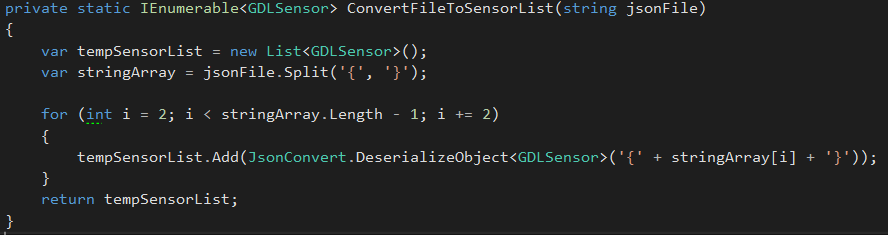
\includegraphics[width=0.8\linewidth]{figs/jsonToSensor}
	\caption{Konvertering fra fil til liste af sensorer.}
	\label{fig:jsonToSensor}
\end{figure}

Denne liste kan vi derefter iterere igennem og indsætte data i databasen.